\documentclass[10pt]{report}

\usepackage[T1]{fontenc}
\usepackage[utf8]{inputenc}
\usepackage[french]{babel}
\usepackage{amsmath}
\usepackage{amsfonts}
\usepackage{amssymb}
\usepackage{graphicx}

\title{INGI2261- AI - Project 3}
\author{Jacquet Charles - 27811200 \\ Degryse Baptiste - 27641200\\ Groupe 34}
\date\today
\begin{document}
\maketitle
\section*{First part}
\subsection*{Question 1}
\begin{center}
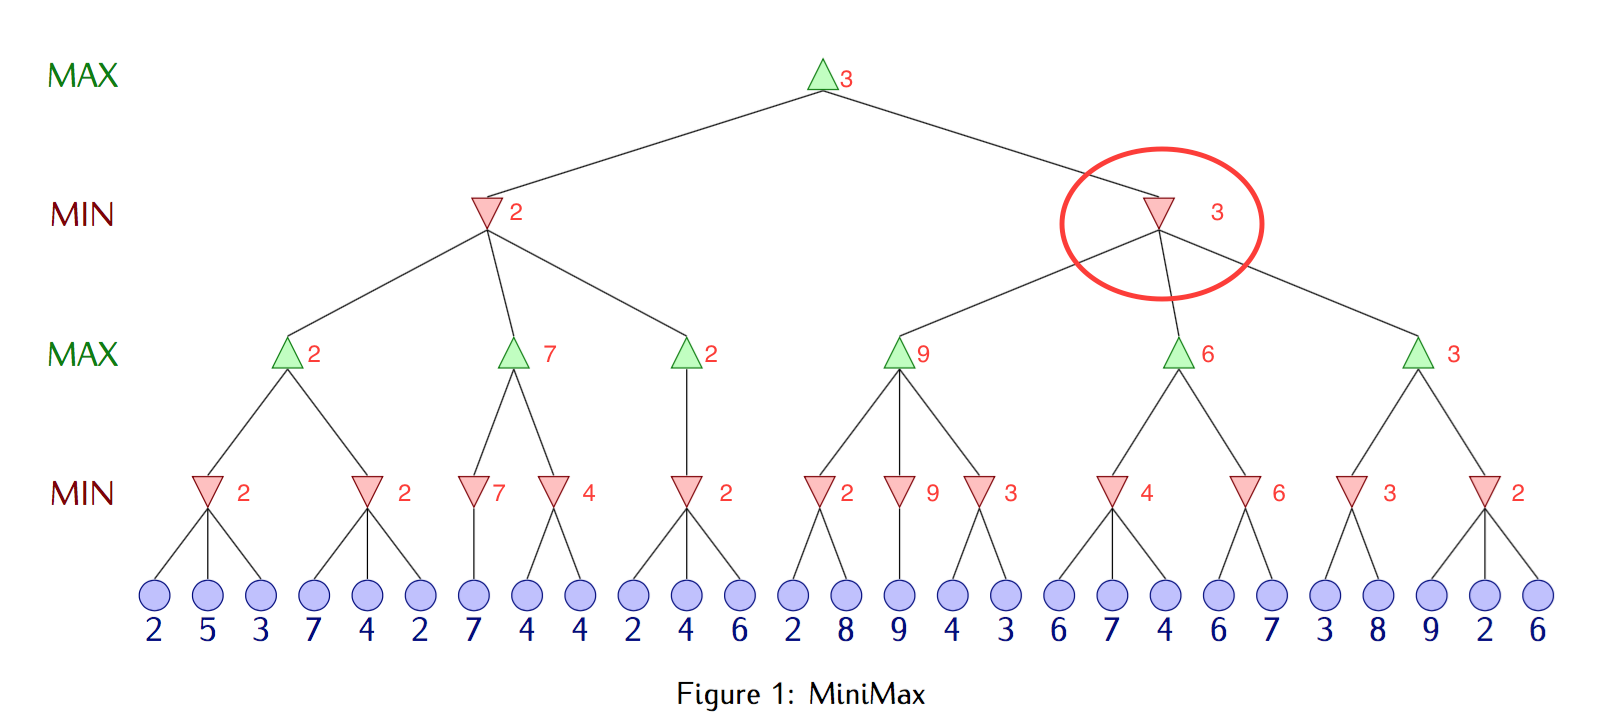
\includegraphics[scale=0.4]{MiniMax}
\end{center}
\subsection*{Question 2}
\begin{center}
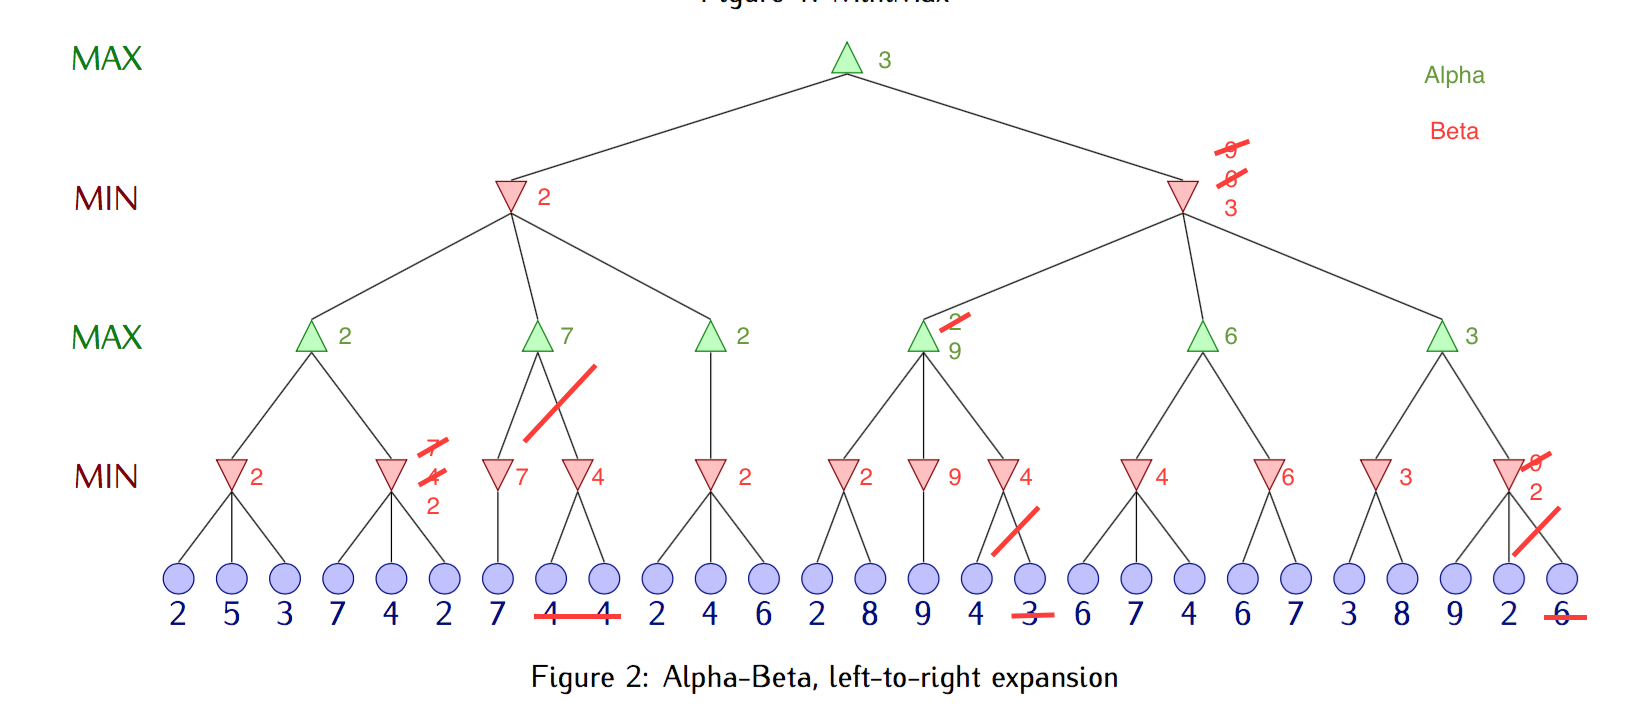
\includegraphics[scale=0.4]{alpha-beta}
\end{center}
\subsection*{Question 3}
\begin{center}
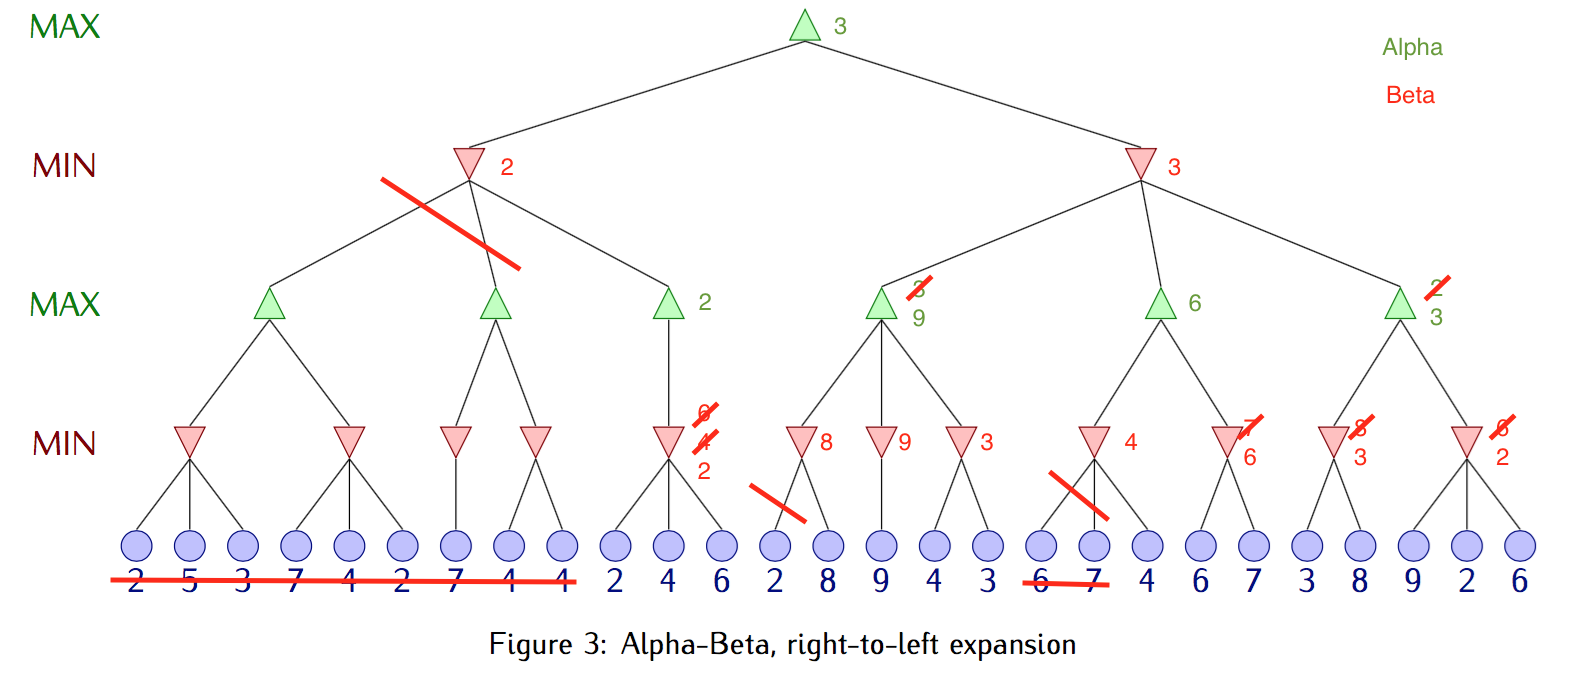
\includegraphics[scale=0.4]{alpha-beta2}
\end{center}
\subsection*{Question 4}
% TO CHECK an do the tree
It's possible if we have the best solution first, then the smallest branching factor.

\begin{center}
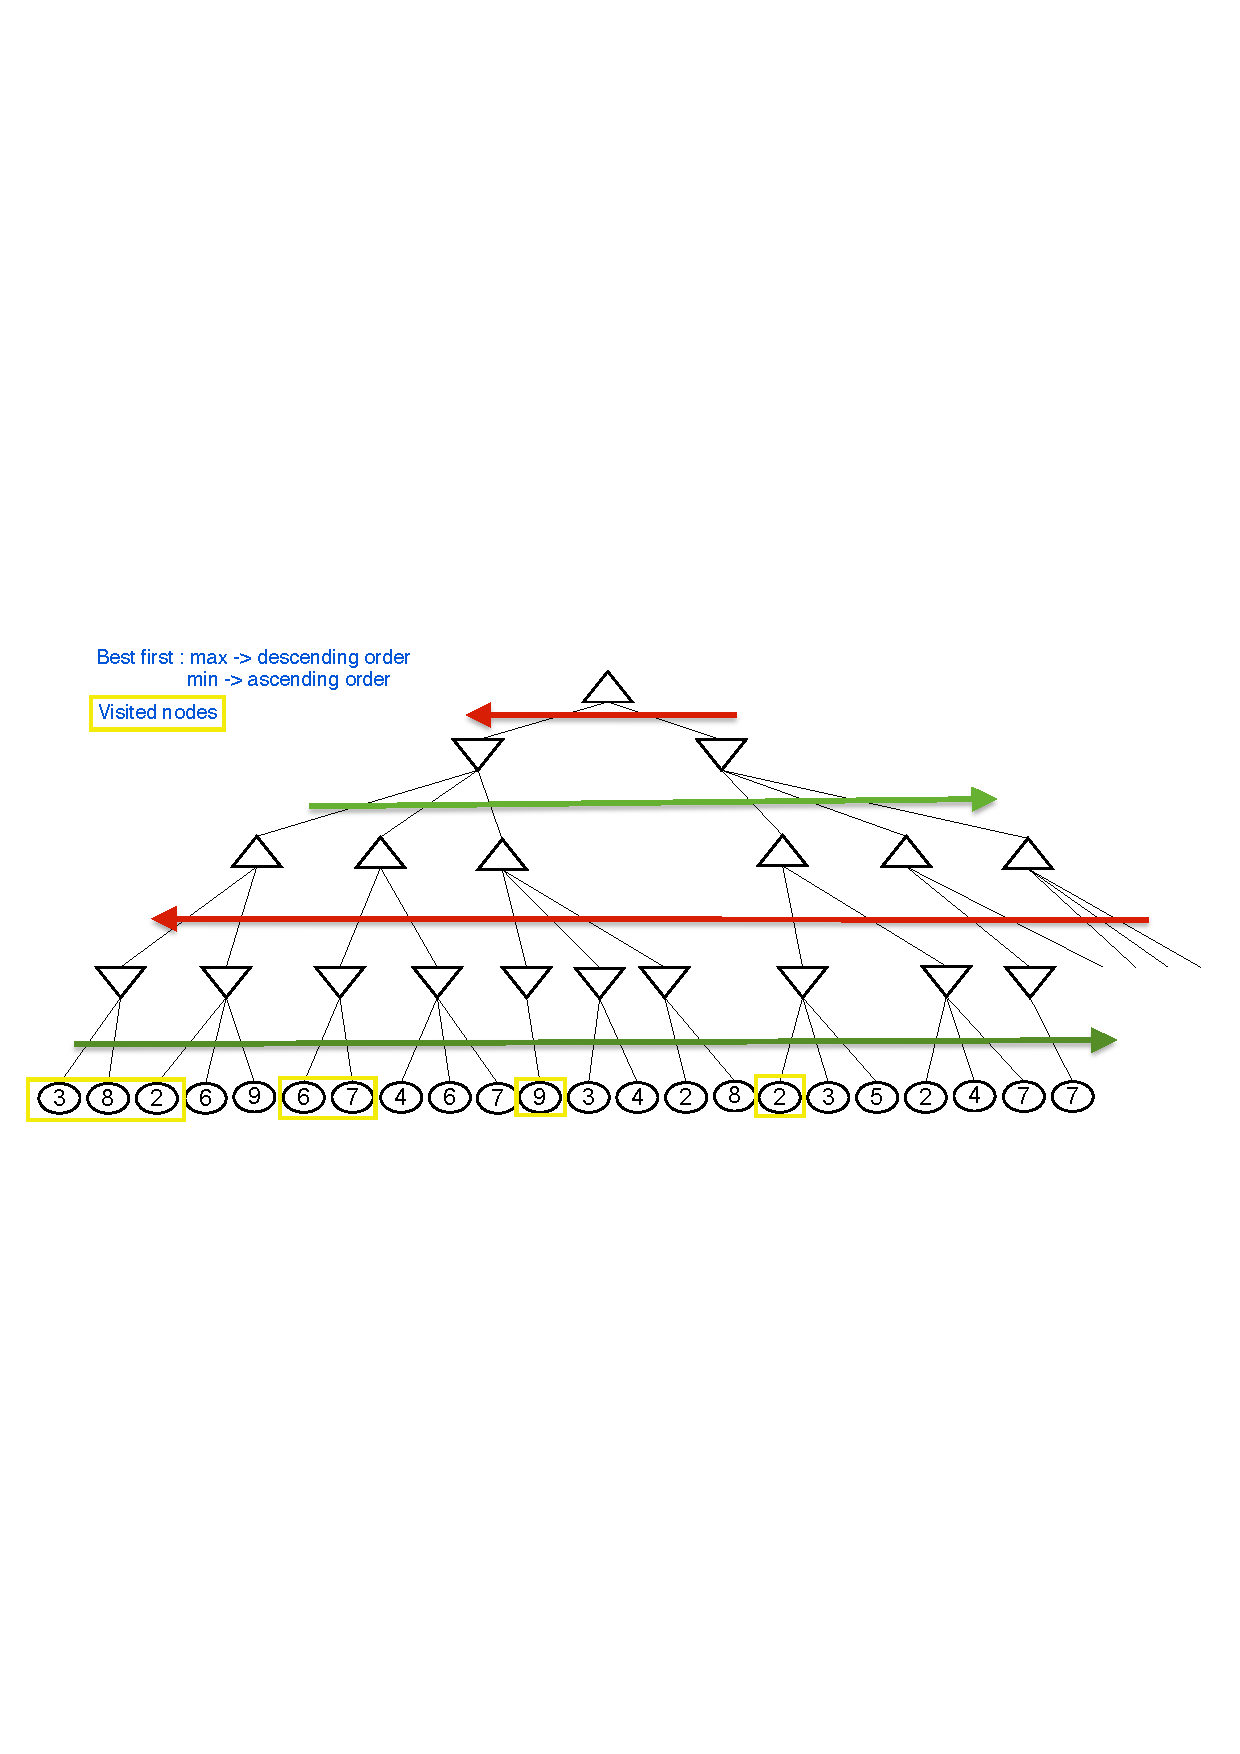
\includegraphics[scale=0.6]{Q4.pdf}
\end{center}

\section*{Second part}
\subsection*{Question 6}
The game shows a fail of the first basic agent. This is due to his incapacity to know how much he wins or fail. So once he leaves the "close to draw" part, his decisions starts to be random. This shows us that the evaluate function needs to use as much nuances as possible (from -100 to 100 rather than from -1 to 1). It's also more efficient due to the fact, that we are doing an alpha-beta pruning. Which is also a kind of MiniMax so the value of the node is important. In the first part, we didn't know which of the « advantageous node » is better than the other so that algorithm take one without any preferences and without being able to prune some nodes.

\subsection*{Question 7}
The evaluate function uses 2 parameters, the color dominance and the safe scores. The safe scores is any tower that cannot move, this includes 5 height towers and isolated piece. The color dominance is just a count of red or yellow towers. The evaluate function return the dominance + 3 times the safe score. We made some test for this factor from 1 to 6 times the safe score, with and without time constraint. The time constraint sometimes reduce the depth of search, and so it changes the result of the tests. The best is 3 with time constraint, but 5 without (always maximal depth)

\subsection*{Question 8}
The upper bound can be found at the game start when the number of possibilities is the highest. Actually, there are 146 possibilities if we want to move a red one and also 146 if we want to move a yellow one which give a total of 292 possibles moves (=branching factor). The lower bound is when the game is finished .. which means there are no valid moves with and then 0 children's state (= branching factor).

\begin{center}
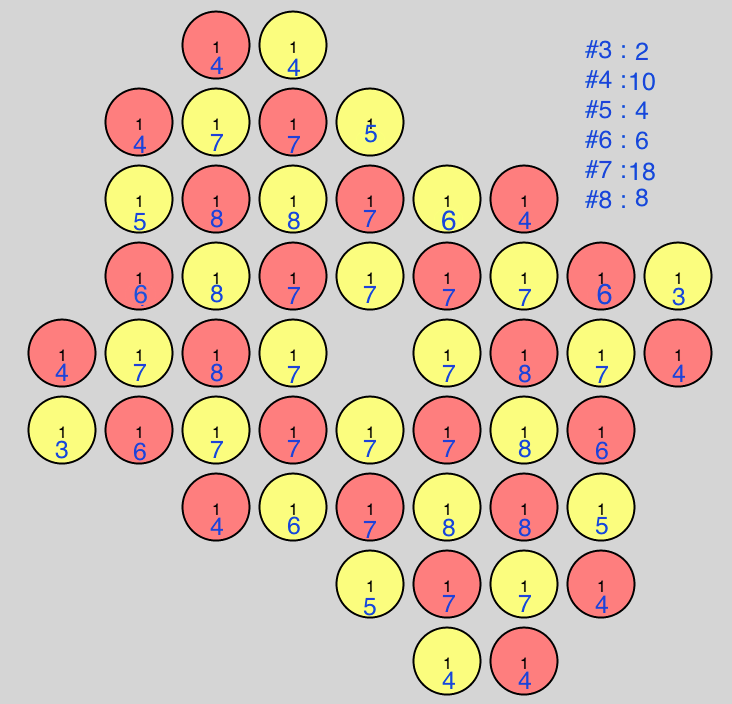
\includegraphics[scale=0.4]{branching.png}
\end{center}

\subsection*{Question 9}
Each move reduces the branching factor by twice the number of neighbors of the moving piece plus the number of new impossible moves due to the new height of the destination piece. The twice is due to the fact that this piece cannot move anymore on the neighbors and the neighbors cannot move on this piece.

\subsection*{Question 10}

Yes, like a human player, we can ignore some successors, but we may miss the best solution (we lose completeness). We have to do this in order to reduce the search time.


\subsection*{Question 11}
Our successors are limited to all the possible moves for all the pieces of a maximum distance of 2 around any towers ( height > 1 ). We chose an arbitrary first move (no towers of height greater than one). We are thinking about changing this by a circle of the n pieces that have the less neighbors (play around isolated towers instead of play around towers). We may use both of these.

\subsection*{Question 12}
The depth represent the numbers of steps from the move that we need to play. We can also say that it is the depth of the tree that we explore looking for the best (depending on the cut-off function) solution. For the minmax algorithm, it's the number of times that we do either the max or the min algorithm.

\subsection*{Question 13}
We need to dynamically chose if we cut-off the search or not. The parameters are the time left depending on the advancement of the game and the depth.

\subsection*{Question 14}
The contest agent implementation had been made thanks to a lot of different tests. We had a lot of ideas but unfortunately it was often bad ideas. And it can be explained by the fact that when we tried to improve the algorithm, we were thinking as human and not as a computer and thus, it doesn't always notice the advantages that we tried to give him ...\\
At first, we began to evaluate the remaining time that we were going to need in average, and if it's too short, we reduce the maximal depth and in other cases, we are using a max\_depth of 3. We also consider a boolean for a short time left in order to be sure to not have time out. This is a reason why we need to be really sure that the best solutions are first in the tree.\\

\begin{center}
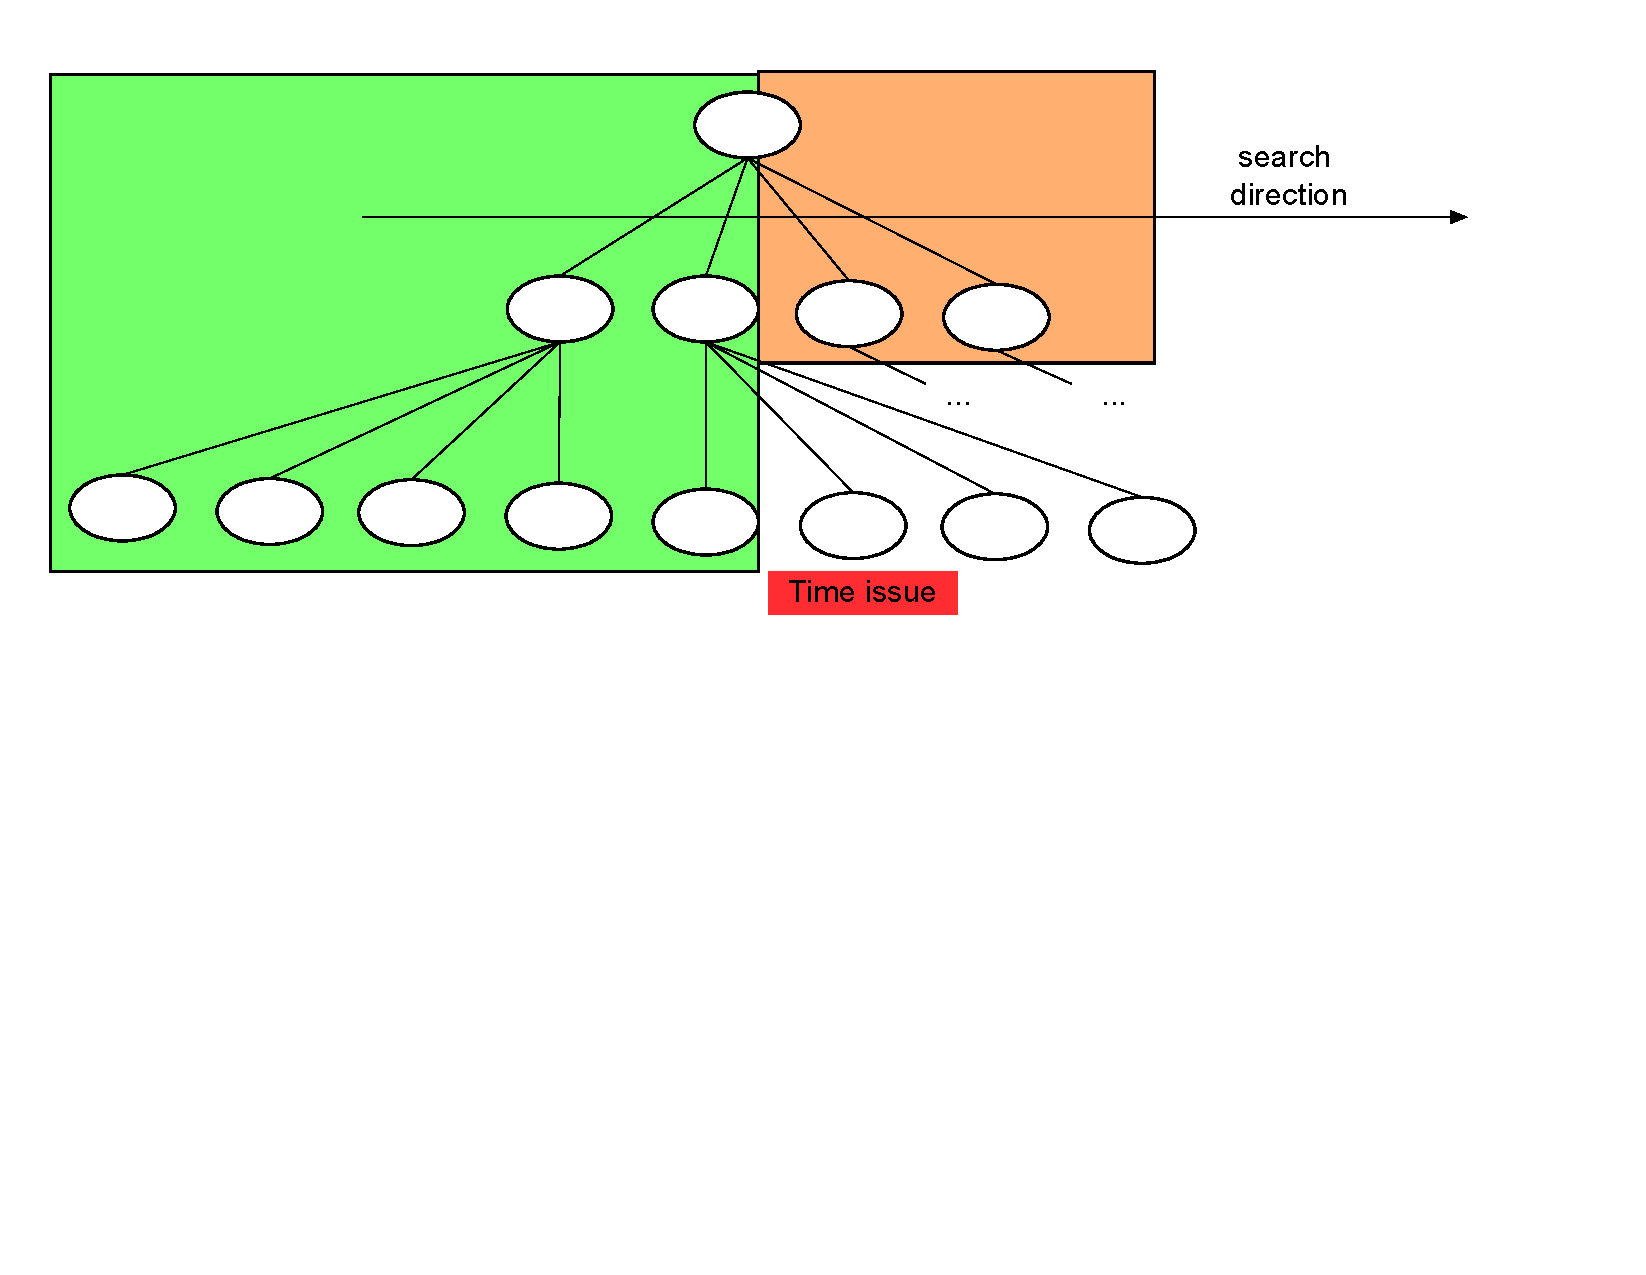
\includegraphics[scale=0.4]{search_with_time.pdf}
\end{center}

But that strategy was not the one that we kept. We have chosen to search on a lot of different nodes even if we can't go really deeper in the search. So, we have a lot of neighbors but the maximum depth that we are looking for the alpha beta algorithm is 3. But if we are close to the end, we have to know that and decrease the depth to avoid possible time out. In order to do so, we are looking the number of considering tower. We than multiplies that by some factors in order to choose if we have to change the max\_depth to 2 or even to 1.\\
An other choice that we have made is to save time in the ten firsts steps by taken a max\_depth of 1 because we always have a lot of other pawns to move around it after so it's not important at first to go farther.\\
Then, we made a lot of try by copying the agent and modifying only one parameter and see which one was winning. When the modification wins in average, we kept this new one. That's how we improved our agent.\\
As already said, we are only considering towers with high over 2 ("big-towers") and then like we know that the game is playing within neighbors of distance 2 from it, we only consider these ones. Then, we decided to give them order, we create 3 lists, tower0 which are the big towers and then tower1 (which has a distance of 1 from tower0) and then tower2 (distance 2). We shuffle each lists (In order to be more efficient against human player) and then, return tower0 + tower1 + tower2. We then realize that an other order 
tower2 + tower1 + tower0 was winning on the first so we have chosen this last one.\\

After all that, we  tried to modify the order of elements that we are checking in order to increase pruning. (if we first check the element that we are going to play, we are sure to do better pruning and so to save time). In order to do that, we have watched our agent playing against itself and saw what were the more played actions. we saw that it's more playing single element towards tower so we put that action in first return (yield) position.\\
At the end, we realize that moves of our IA are often really not the best moves that it could do .. We decided so to modify the way that we've implemented our evaluate function. To do so, for each move, we "give points" in function of a ratio: the number of our color neighbors divided by the number of neighbors with the opponent color.\\
 Because getting a tower surrounded with our color is nearly always a better move.

\end{document}
